% Chapter 1

\chapter{Background Theory} % Main chapter title

\label{Chapter1} % For referencing the chapter elsewhere, use \ref{Chapter1} 

%----------------------------------------------------------------------------------------

% Define some commands to keep the formatting separated from the content 
\newcommand{\keyword}[1]{\textbf{#1}}
\newcommand{\tabhead}[1]{\textbf{#1}}
\newcommand{\code}[1]{\texttt{#1}}
\newcommand{\file}[1]{\texttt{\bfseries#1}}
\newcommand{\option}[1]{\texttt{\itshape#1}}

%----------------------------------------------------------------------------------------

\section{Artificial Neural Networks}
Artificial neural networks are parallel distributed processing systems that are composed by  neurons, their most elementary building block. Neurons are processing  units that generate an output according to an activation function $\phi(x)$, which is usually a sigmoid function like in equations \ref{eq:1} and \ref{eq:2}.\\

Logistic Regression: 

\begin{equation}\label{eq:1}
\phi(h)= \left\{
			 \begin{array}{ll}
			 	1, h\geq0\\
			 	0, h<0
			\end{array}
		 \right.
\end{equation}


Hyperbolic tangent function:

\begin{equation}\label{eq:2}
\phi(h)=tanh(h)
\end{equation}
\\

Neurons are interconnected by links, and the arrangement of these links determine different types of neural networks. If the links are cyclical for example, the neural network is considered recurrent. The synaptic links between the neurons also have strengths that are coded by weights. 
\\
Figure~\ref{fig:Neuron} shows a mathematical model given by [\cite{Reference2}] of a neuron, with $j1$ input signals $x_1, x_2, ..., x_{j1}$ and an output signal $y$. This model also shows the weights of each of the input links of this neuron as $w_1, w_2,...,w_{j1} $, a bias term $\Theta$ and an activation function $\phi(x)$. The output of this neuron is the aggregation of the input signals, shifted by the bias term and processed by the activation function; as shown in equation \ref{eq:3}.

\begin{figure}[h]
	\centering
	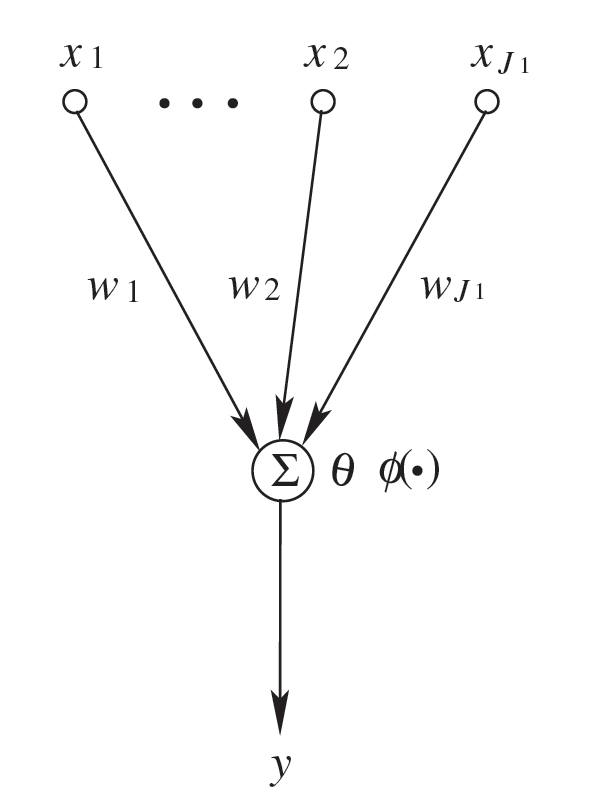
\includegraphics{Figures/neuron_mathematical_model.PNG}
	\decoRule
	\caption[Mathematical Model of a Neuron]{Mathematical Model of a Neuron.}
	\label{fig:Neuron}
\end{figure}

\begin{equation}\label{eq:3}
	y=\phi(input + bias)=\phi(W^{T}X-\Theta)=\phi(\sum_{i=1}^{J1} w_i x_i - \Theta)
\end{equation}
%----------------------------------------------------------------------------------------

\section{Challenges in RNNs}
It has been theoretically proven that RNNs can be universal approximators of dynamic systems [\cite{Reference1}], which represents a powerful potential for modeling natural systems more accurately compared to existing methods such as FNNs. However, practical applications of RNNs have been stagnated due to theoretical and implementation challenges encountered in the this model. This section specifies some of these challenges. 

\subsection{Computational Cost}
High computational cost for non-linear activation functions such as sigmoid functions.

\subsection{Supervised Training}
Supervised training is very difficult


%----------------------------------------------------------------------------------------

\begin{flushright}
Guide written by ---\\
Sunil Patel: \href{http://www.sunilpatel.co.uk}{www.sunilpatel.co.uk}\\
Vel: \href{http://www.LaTeXTemplates.com}{LaTeXTemplates.com}
\end{flushright}
